\question Draw out a box-and-pointer diagram for the following list:

\begin{lstlisting}[language=Scheme]
scm> (define nested-lst (list 1 (cons 2 (cons 3 'nil)) '(4 5 6) 7))
nested-lst
\end{lstlisting}
\begin{solution}[1.25in]
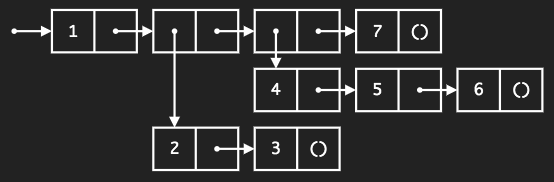
\includegraphics[scale=.7]{../topics/scheme/images/nested-lst.png}
\end{solution}

Then, write out what Scheme would display for the following expressions:

\begin{lstlisting}[language=Scheme]
scm> (cdr nested-lst)
\end{lstlisting}
\begin{solution}[0.15in]
\begin{lstlisting}[language=Scheme]
((2 3) (4 5 6) 7)
\end{lstlisting}
\end{solution}

\begin{lstlisting}[language=Scheme]
scm> (cdr (car (cdr nested-lst)))
\end{lstlisting}
\begin{solution}[0.15in]
\begin{lstlisting}[language=Scheme]
(3)
\end{lstlisting}
\end{solution}

\begin{lstlisting}[language=Scheme]
scm> (cons (car nested-list) (car (cdr (cdr nested-list))))
\end{lstlisting}
\begin{solution}[0.15in]
\begin{lstlisting}[language=Scheme]
(1 4 5 6)
\end{lstlisting}
\end{solution}
